\chapter{Introduction}\label{cap.introduccion}

\setlength{\parindent}{0pt}
The Multiple Object Tracking or \textit{MOT} is an important computer vision problem which continues to attract attention because of its potential in both the academic and commercial spheres. The real-world applications of the multiobject tracking are numerous including human-computer interaction, autonomous vehicles, robotics, video indexing, surveillance or security, among others. Many autonomous car projects are taking place globally which require solutions to various different problems including to keep an eye to all other moving objects in the area where the car is located (Figure \ref{fig:adas_tracking}). The outputs from the tracking module are a basic input for other modules like maneuver planning and trajectory planning. Autonomous vehicles are key in the continuous contribution of the progress made in tracking, and in the computer vision community in general. Many multi-object tracking algorithms have been proposed to solve the problem of real-world traffic monitoring where algorithms have to deal with complex occlusion situations and difficult object matching.\\
In an era where human-computer interaction has become particularly important due to the quick development of touch display technology available in every smartphone the hand is of big interest. The object tracking is an important part of this area. For example, it is being used for tracking the hand movements because of its non-intrusive nature compared to other types of sensing which could imply the user to wear gloves, among others. With this tracking we can develop very interesting applications that range from predicting sign language to games like playing ``hand ping pong".
\\
The computer vision community have been making big efforts in the past few decades to solve the MOT problem but the task is still open for improvement. One of the most studied tracking areas is the pedestrian tracking, mainly because this particular kind of object can be seen in a large number of applications with commercial potential. As some studies indicate [1], about the 70\% of the current research done in MOT is dedicated to pedestrians. The difficulty of MOT lies in various challenging situations that can occur such as variation of the illumination, variation of scale, target deformation or fast motion. Most of this challenges are common to Single Object Tracking (\textit{SOT}) but MOT also needs to solve two main tasks: determining the number of objects and mantaining its identities over the time.\\
\begin{figure}[h!]
\begin{center}
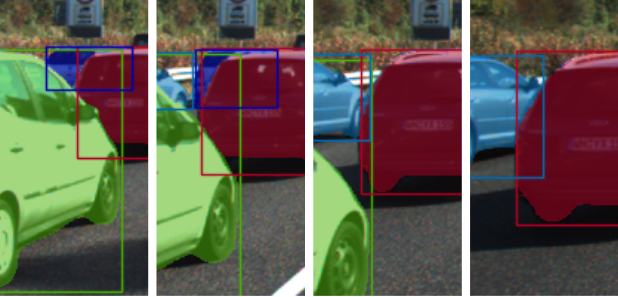
\includegraphics[scale=0.4]{figures/adas_tracking.png}
\caption{The importance of tracking in the autonomous vehicles \cite{voigtlaender2019mots}}
\label{fig:adas_tracking}
\end{center}
\end{figure}\\
In the \textit{Artificial Intelligence} era the multi-object tracking makes use also from the AI to improve the tracking algorithms. One of the most well known and currently growing subfields in AI is \textit{Deep Learning}. These techniques are being used for a broad range of applications such as object detection, image classification, biometrics or medical imaging, among others (Figure \ref{fig:ssd_detection}). In most cases, the Deep Learning has beaten the current State-of-the-Art in these areas.\\
A popular example of image classification is the case of classifying a handwritten digit (multiclass classification) from the MNIST dataset. Numerous applications can surge from recognizing digits and numbers like the automated recognition of house numbers in Google Street View images (Figure \ref{svhn}).
\begin{figure}[H]
\begin{center}
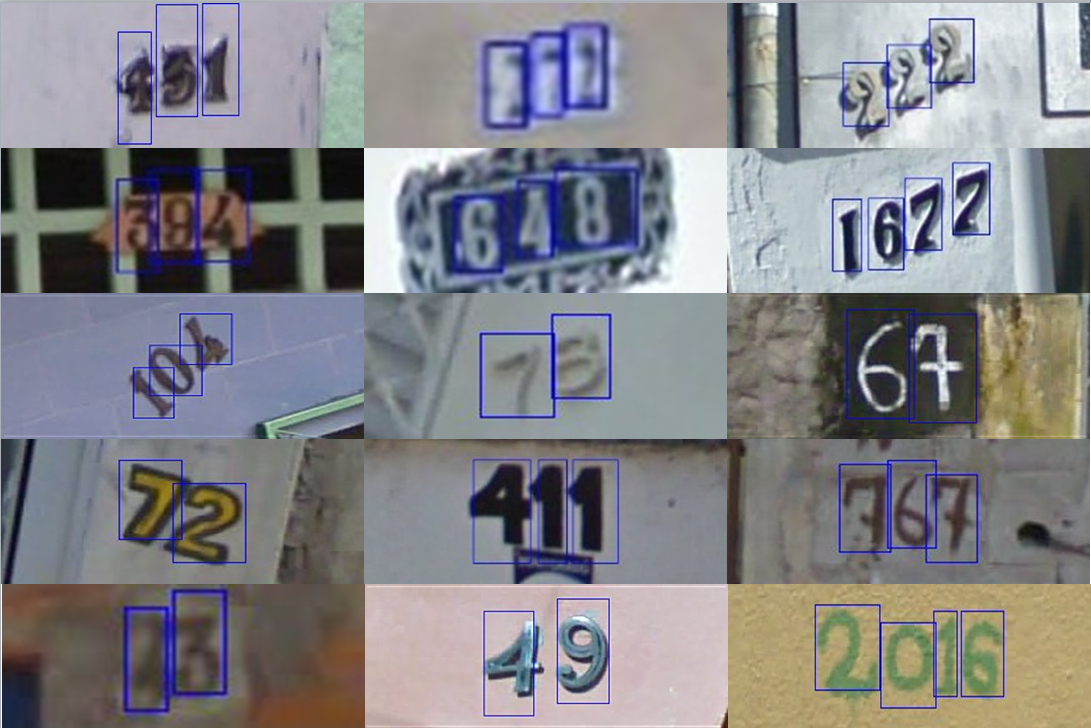
\includegraphics[scale=0.3]{figures/svhn.png}
\caption{Digit recognition on SVHN dataset \cite{netzer2011reading}}
\label{svhn}
\end{center}
\end{figure}
Apart from the typical deep learning applications, in the last few years other applications that can be tagged as ``artistic" have emerged like, for example, the style transfer. The neural style transfer consists on learning the style from one or more images and applying that style to a new image. This can give some very interesting results as it can be seen in Figure \ref{style_transfer}. There are other examples of ``artistic" deep learning such as image colorization using deep learning. In this case the neural colorization tries to convert a grayscale image to a color image which can be very helpful in areas like photography or cinema.
\begin{figure}[H]
\begin{center}
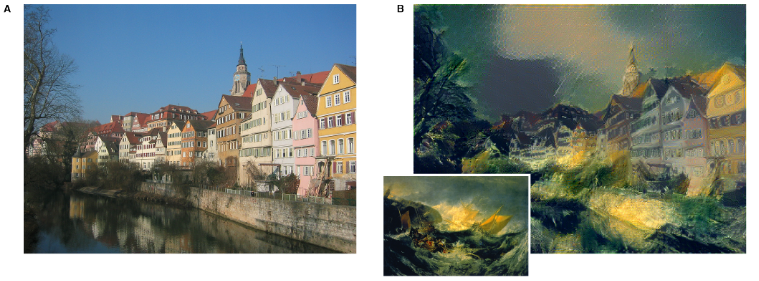
\includegraphics[scale=0.4]{figures/style_transfer.png}
\caption{Example of neural style transfer from famous artworks to a photograph \cite{gatys2015neural}}
\label{style_transfer}
\end{center}
\end{figure}
Given the broad areas of application where deep learning is succeeding and the ones who are still in research it is going to be studied on this master thesis the use of deep learning techniques to tackle the multi-object tracking problem.
\begin{figure}[H]
\begin{center}
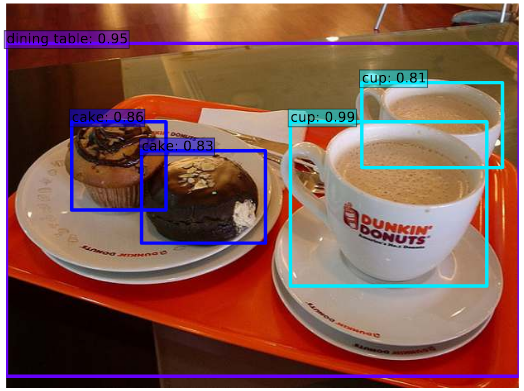
\includegraphics[scale=0.35]{figures/ssd_detection.png}
\caption{Object detection using deep learning techniques \cite{liu2016ssd}}
\label{fig:ssd_detection}
\end{center}
\end{figure}
The deep learning for tracking has been used in previous works from other colleagues such as Marcos\footnote{\href{https://gsyc.urjc.es/jmplaza/students/tfm-visualtracking-marcos_pieras-2017.pdf}{Visual people tracking with deep learning
detection and feature tracking}}. In his work, the task is a visual tracking on people using deep learning with a classical feature tracking based on the Lucas-Kanade algorithm. The detections obtained by the neural networks allow to build a robust hybrid tracker. However, this detections are precalculated before launching the tracking.\\
Other interesting works with neural networks, in this case, for object detection have been developed such as \textit{Object Detector}\footnote {\label{object_detector}\href{https://github.com/JdeRobot/dl-objectdetector}{Object Detector}}.
This application is composed of 3 entities working with an asynchronous design as threads. The entities are a \textit{Camera} that provides the images, a \textit{GUI} that provides the user interface and a \textit{DetectionNetwork} that encapsulates an object detector neural network. As a result this node allows the user to visualize object detections, i.e.\ bounding boxes drawn over the image in real-time. The images can be obtained from different sources as a webcam, a video or via remote proxy. It also provides functionality to perform on-demand detection when preferred. The Figure \ref{fig:object_detector} shows the Object Detector running.
\begin{figure}[H]
\begin{center}
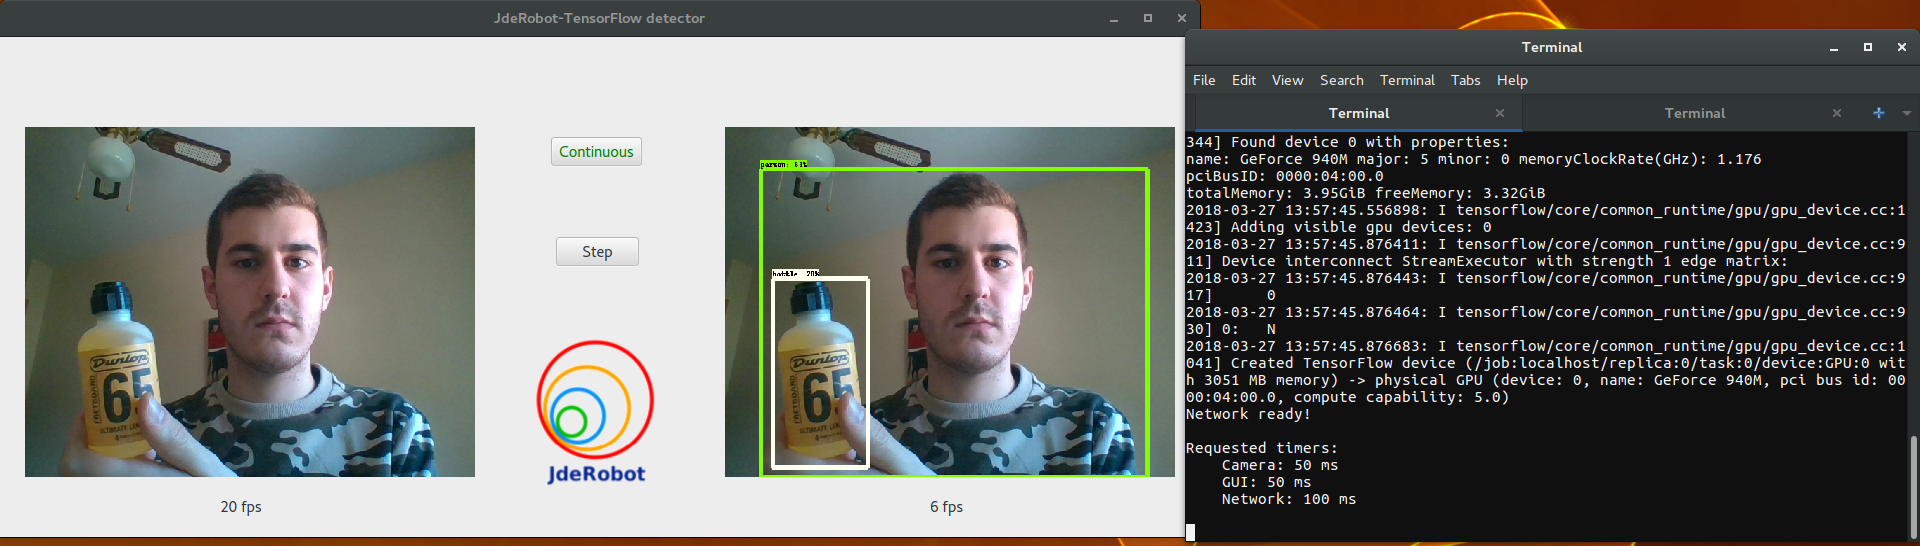
\includegraphics[scale=0.25]{figures/object_detector.png}
\caption{Example of the Object Detector node working in real-time (from \ref{object_detector})}
\label{fig:object_detector}
\end{center}
\end{figure}
The user can download pre-trained open neural network models for \textit{Tensorflow} or \textit{Keras} and configure the Object Detector to work with them.\\
As it has been seen, the deep learning and the multiobject tracking are still open areas where multiple applications can be obtained.\\
\section{Objectives}
After the introduction of the context of the work has been made, in this section we will explain the main objectives of this thesis and the methodology used to fulfil them.
\\
The main objective of this master thesis is to build a multi-object tracking application which makes use of two techniques: deep learning and tracking by detection. In this work we are going to study how to use the best of both techniques to build a multiobject tracker which can be capable of run in resources constrained hardware on simulated real-time. This work takes the form of a user application and allows multiple configurations. For this reason, the available solutions are going to be tested in well-known datasets of multiobject tracking challenges which will provide the performances obtained by each configuration of the application. This allows the selection of the best configuration.\\
This task can be divided into different subobjectives:
\begin{itemize}
\item \textbf{Object detector using deep learning}\\
Learn the fundamentals of object detection using deep learning techniques. Study the performance on both accuracy and speed of these techniques in datasets. Finally, select the default object detector.
\item \textbf{Development of the tracking module}\\
Build the tracking module taking into account the necessity of speed in constrained resources.
\item \textbf{Threads infraestructure and synchronization}\\
Integration of the modules needed into a thread infrastructure. This will imply a sophisticaded synchronization between them.
\item \textbf{Test the application}\\
Finally, validate the solutions obtained and select the best configuration based on the results.
\end{itemize}

\section{Methodology} \label{Methodology}
The development of this project has been weekly followed by the tutor. In this weekly meetings the work done in the previous week was evaluated and discussed ending in new milestones for the following week. This continuous feedback allowed a better development of the project both in terms of understanding of the topic and in terms of time.\\
Apart from that, the following tools have been employed to follow the project progress and making it visible for the community:
\begin{itemize}
    \item \textbf{GitHub:} the code of the project is available on GitHub and was constantly updated. The repository can be accessed in the following link: \url{https://github.com/RoboticsURJC-students/2017-tfm-alexandre-rodriguez}
    \item \textbf{Wiki:} it has been used as a logbook of the progress of the project. In \url{http://jderobot.org/Arodriguez-tfm} the steps followed to achieve this target can be seen.
\end{itemize}
